\documentclass{book}
\usepackage{amsmath, amsthm, amssymb, amsfonts}\usepackage{thmtools}\usepackage{parskip}\usepackage[pdftex]{graphicx}\usepackage[a4paper, margin=4cm]{geometry} % margins%
\usepackage{calc}\usepackage{setspace}\usepackage{geometry}\usepackage{float}\usepackage[hidelinks]{hyperref}\usepackage[utf8]{inputenc}\usepackage[english,danish]{babel}\usepackage{framed}\usepackage[dvipsnames]{xcolor} \usepackage{tcolorbox}\usepackage{hyperref}\usepackage{lastpage}\usepackage{fancyhdr} \usepackage{afterpage}
%https://www.overleaf.com/learn/latex/Multiple_columns Linket her kan bruges til at indelle sider i kolumner
\usepackage{titlesec} %den her pakke bruges til at fjerne "Kapitel n" fra kapitelsidderne
\usepackage{minitoc}
\titleformat{\chapter}[display] {\normalfont\huge\bfseries}{}{0pt}{\Huge} \pagestyle{fancy}
\fancyhf{} % Clear the header and footer
\fancyhead[LE,RO]{\thepage} % Page number on the outer (left on even, right on odd) side
\fancyhead[RE]{\leftmark} % Chapter title on the inner side (right on even pages)
\fancyhead[LO]{\leftmark} % Chapter title on the inner side (left on odd pages}
\title{Victors Kogebog med Stjålne Opskrifter}
\author{Victor Posselt Sandberg}
\date{\today}
\renewcommand{\chaptermark}[1]{\markboth{#1}{}} % Fjerne kapitel nummeret fra headeren
\usepackage{tikz}

\begin{document}
\dominitoc  

\frontmatter
%\maketitle 
\titlepage % Output the title page
	{
\includegraphics[width=\paperwidth]{background.pdf} % Code to output the background image, which should be the same dimensions as the paper to fill the page entirely; leave empty for no background image
	{ % Title(s) and author(s)
		\centering\sffamily % Font styling
		{\Huge\bfseries Victors Kogebog med Stjålne Opskrifter\par} % Book title
		\vspace{16pt} % Vertical whitespace
		{\LARGE A Practical Guide\par} % Subtitle
		\vspace{24pt} % Vertical whitespace
		{\huge\bfseries Goro Akechi\par} % Author name
	}

\begin{figure}
    \centering
    
\includegraphics[width=1\linewidth]{Mave2.jpg}
    \caption{Det mig}
    \label{fig:enter-label}
\end{figure}
\newpage \tableofcontents
\mainmatter
\newpage\chapter{Introduktion} \doublespacing
Gennem de sidste 2 år har jeg haft til mål at lave mindst en ny opskrift hver måned. Dette har inspireret mig til at lave en masse nye, anderledes og lækre ting. Det har også bragt mig til den opdagelse at det er svært at finde på noget nyt hver måned, så nu vil jeg prøve at samle alle de opskrifter jeg har fundet og lavet i min jagt. Mange af opskrifterne er fundet på valdermersro, men nogle af dem (nogle af de lidt mere ekstraordinære) kommer fra andet steds, eller endda hvad jeg har kunne finde på at skrue sammen af resterne i køleskabbet. Jeg håber at denne bog kan give inspiration til, enten selv at opstille et ligende mål, eller blot giver en lækker aftensmad eller 2\text{;)} 
\singlespacing
\chapter{Morgenmad}
\section{Brunch}
\underline{Røræg}
\\ - 4 æg
\\ - 100 g cremfraice eller græsk yoghurt
\\ Salt, pebber og evt. timian
\\ \textbf{Fremgansmåde:}
\\ Bland æggne og mælkeproduktet sammen til en ens formig masse og steg på panden ved lav varme. Der kan med fordel vendes med en spise pind da det giver mindre smuldrende æg.


\chapter{Frokost} 
\section{Couscous salat}
\begin{minipage}[t]{0.5\textwidth}
\end{minipage}
\begin{minipage}[t]{0.5\textwidth}
\end{minipage}
\chapter{Ikke Vegetarisk Aftensmad} 
\minitoc
\newpage \section{Bibimbap}
\begin{minipage}[t]{0.5\textwidth}
    \textbf{Ingredienser:}
    \begin{itemize}
        \item Sovs
        \begin{enumerate}
            \item 2 dele Gochujang (koreansk chilli paste)
            \item 2 dele sesam olie 
            \item 2 dele Soja sauce
            \item 1 del sukker eller brun farin
            \item 0.5 del hvidvin eller æbleeddike
        \end{enumerate}
        \item Grøntsager og tilbehør
        \begin{enumerate}
            \item Spidskål
            \item Gulerøder
            \item Bønnespirer 
            \item Svampe (Champignioner eller Porto Bello)
            \item Spinat 
            \item Spejlæg
            \item Ris
        \end{enumerate}
    
        \item Kød
    \end{itemize}
        \begin{enumerate}
            \item Oksekød (enten hakket oksekød eller flanksteak)
        \end{enumerate}
\end{minipage}
\begin{minipage}[t]{0.5\textwidth}
\textbf{Fremgangsmåde}    
\begin{enumerate}
    \item Til at starte
\end{enumerate}
\end{minipage}
\newpage \section{Butter Chicken}
\begin{minipage}[t]{0.5\textwidth}
\end{minipage}
\begin{minipage}[t]{0.5\textwidth}
\end{minipage}
\section{Carbonarra}
\begin{minipage}[t]{0.5\textwidth}
\end{minipage}
\begin{minipage}[t]{0.5\textwidth}
\end{minipage}
\section{Flæskesteg}
\begin{minipage}[t]{0.5\textwidth}
\end{minipage}
\begin{minipage}[t]{0.5\textwidth}
\end{minipage}
\newpage \section{Fruta de Mer}
\begin{minipage}[t]{0.5\textwidth}
\textbf{Ingredienser:}
\begin{itemize}
    \item250g Pasta(jeg fortrækker en form for linguinne)
    \item250g arabiatta sauce (Variende alt efter hvor tomattet den skal være)
    \item500g Skaldyr(rejer,blåmuslinger og hvad man ellers lige har lyst til)
    \begin{enumerate}
        \item evt. laks
    \end{enumerate}
    \item Persille og citron til servering
\end{itemize}
\end{minipage}
\newpage
\begin{tikzpicture}[remember picture,overlay,inner sep=0pt,outer sep=0pt]
    \node[anchor=south east] at (current page.south east) {
        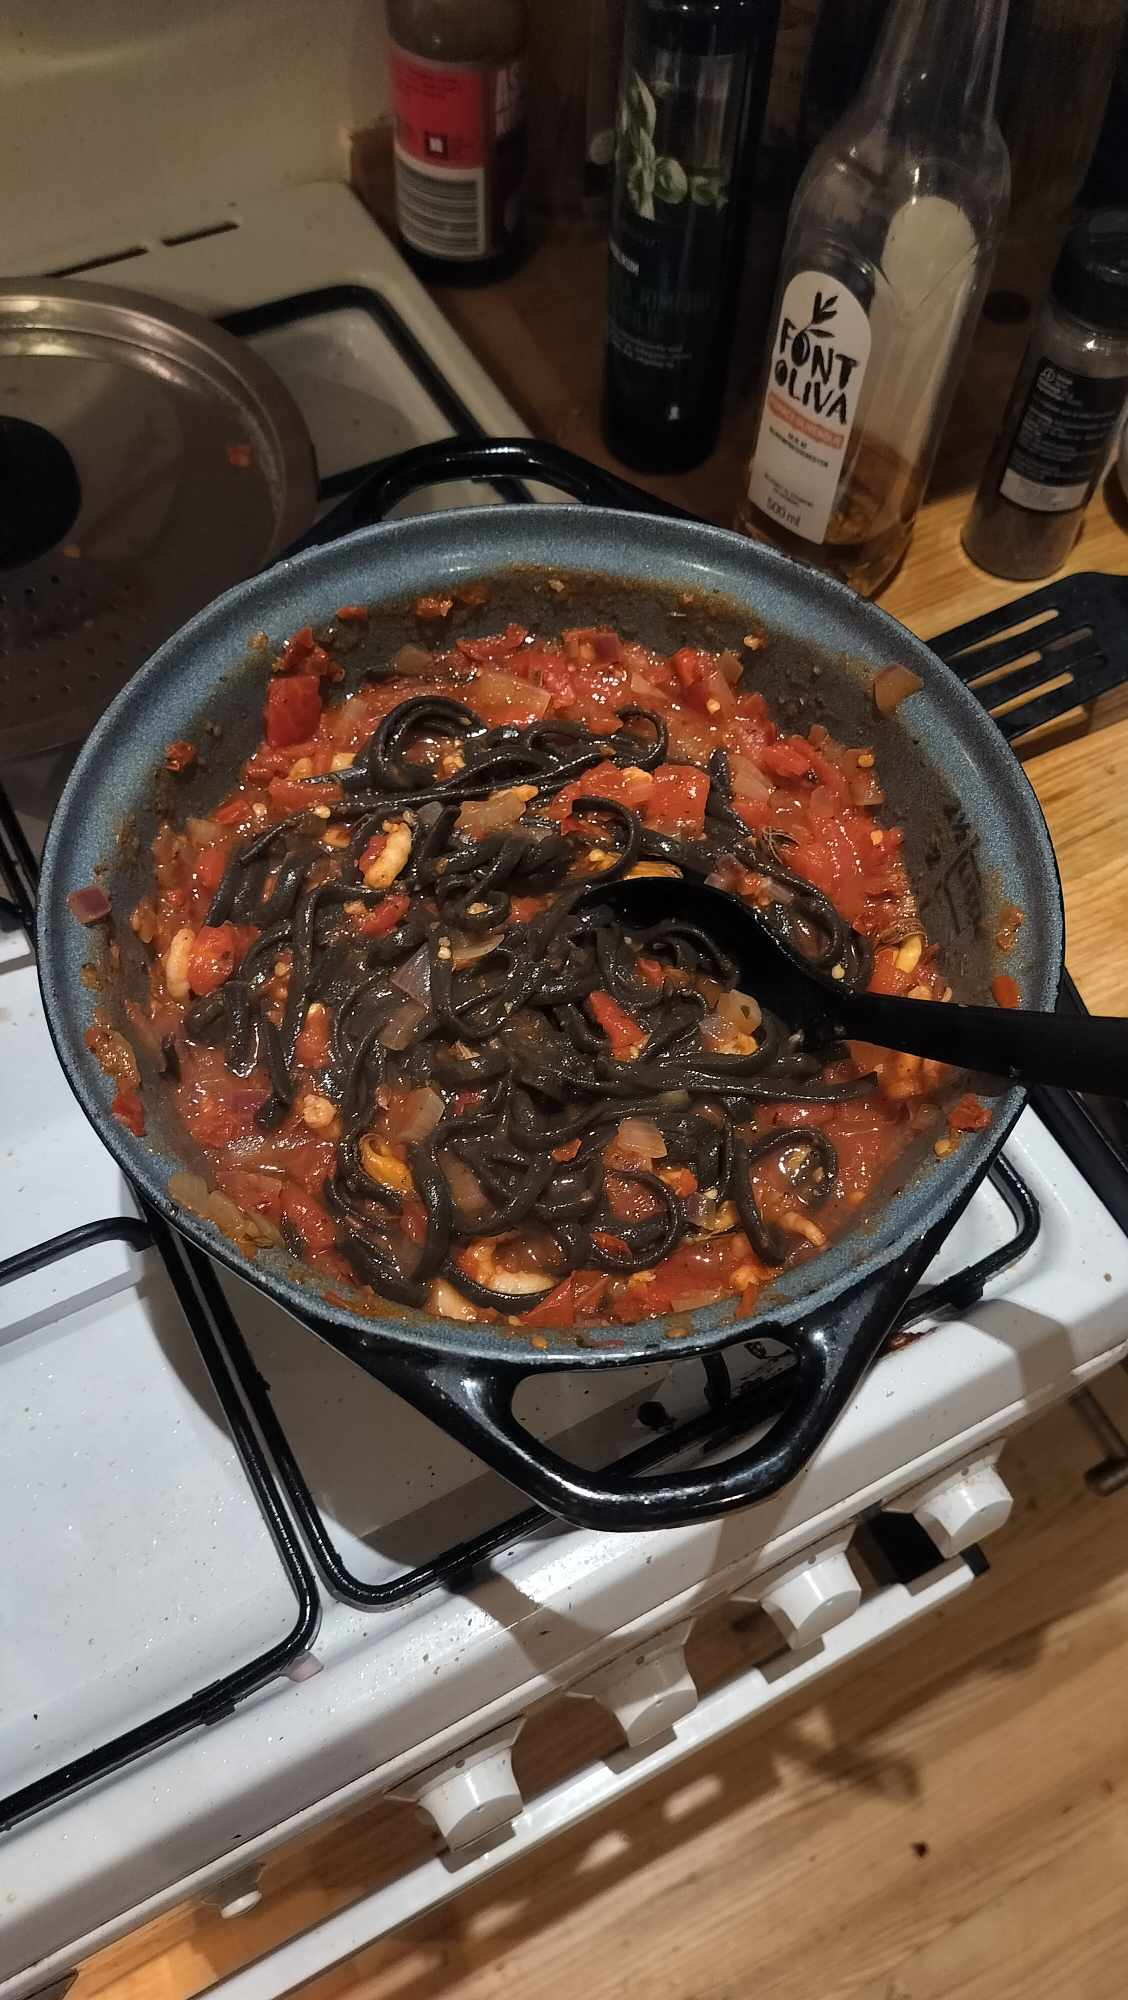
\includegraphics[width=\paperwidth,height=\paperheight]{Fruta_de_mer.jpg}
    };
\end{tikzpicture}
\newpage \section{Stegte Ris}
\begin{minipage}[t]{0.5\textwidth}
\begin{itemize}
    \item 200g kogte ris
    \item 200g blandede grøntsager
    \item 100g mukimamme bønner
     \begin{enumerate}
        \item evt. Flere grøntsager hvis ønskede
        \item evt. Pandestegt spidskål (eventuelt stegt i goyang(koreansk chille pasta))
    \end{enumerate}
    \item 100g kylling
    \item soja til stegning
    \item 1 æg til stegning
\end{itemize}
\end{minipage}
\begin{minipage}[t]{0.5\textwidth}
\end{minipage}

\newpage \section{T'uhu}
Sumerisk lam og rødbede gryderet, som er den ældste kendte opskrift, estimeret at være flere tusind år gammel.

\begin{minipage}[t]{0.5\textwidth}
\textbf{Ingredienser:}
\begin{itemize}
    \item 500g Fedtrigt lam i tern (Egentlig fårkød men det pænt svært at få)
    \item 100 mL Fårfedt (eller kokosolie)
    \item 1 løg
    \item 1 tsk salt
    \item 500g Rødbedder i tern
    \item 100g hakket rucola
    \item Frisk koriander
    \item 125g hakket skalotteløg
    \item 1 tsk spidskommen frø
    \item 100mL Weissbier
    \item 50 mL vand
    \item 75g hakket porrer
    \item 3 fed hvidløg
\end{itemize}
\underline{Tilbehør:}
\begin{itemize}
    \item 75g friske hakkede koriander
    \item 75g forårsløg
    \item 2 tsk spidskommen frø
\end{itemize}
\end{minipage}%
\begin{minipage}[t]{0.5\textwidth}
\textbf{Fremgangsmåde:}
\begin{enumerate}
    \item Varm kokosolie (eller andet fedt) i en gryde bred nok til det hakkede lam, i et lag.
    \item Svitser lammet indtil al væsken er væk.
    \item Tilsæt løgene og steg indtil de er gennemsigtige.
    \item Tilsæt derefter salt, rødbeder, rucola, koriander, skalotteløg og spidskommenfrø, og steg indtil væsken er væk.
    \item Tilsæt ølen, vandet og bring det i kog.
    \item Tilføj løg og porrer og lad det simre i en times tid.
\end{enumerate}
\underline{Tilbehør:}
\begin{enumerate}
    \item Knus foråsløgene og korianderne i en morter eller lignende og drys spidskommenfrøene på.
\end{enumerate}
\end{minipage}
\enlargethispage{\baselineskip}
\footnote{Kilde: \href{https://www.bbc.com/travel/article/20191103-the-worlds-oldest-known-recipes-decoded}{BBC travel}}
\newpage
\begin{tikzpicture}[remember picture,overlay,inner sep=0pt,outer sep=0pt]
    \node[anchor=south east] at (current page.south east) {
        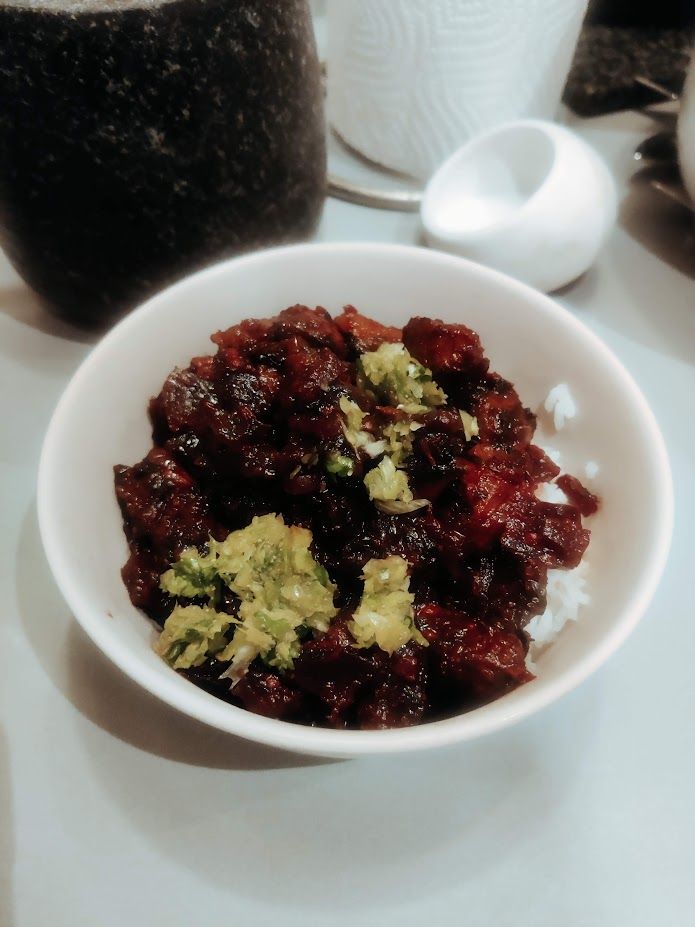
\includegraphics[width=\paperwidth,height=\paperheight]{Tuhu.jpg}
    };
\end{tikzpicture}


\chapter{Vegetarisk Aftensmad}
\section{Arabiatta}
\begin{minipage}[t]{0.5\textwidth}
\end{minipage}
\begin{minipage}[t]{0.5\textwidth}
\end{minipage}
\newpage \section{Dhal}
\begin{minipage}[t]{0.5\textwidth}
\textbf{Ingredienser} \\
\underline{Dhal}
\begin{itemize}
    \item 4 fed hvidløg
    \item 2 løg
    \item 2 spsk frisk revet ingefær, eller 2 tsk tørret
    \item 2 spsk olivenolie
    \item 200 gram tørre røde linser
    \item 2 dåser hakkede tomatter
    \item Kryderier
    \begin{enumerate}
        \item 6 dL grøntsagsbouillon
        \item 0.5 tsk chiliflager
        \item 0.5 tsk stødt kardemonne
        \item 0.5 spsk stødt koriander
        \item 1 spsk stødt spidskommen
        \item 0.5 tsk garam masala
        \item 0.5 tsk paprika
    \end{enumerate}
    \end{itemize} 
\underline{Raita:}
\begin{itemize} 
    \item 1 håndfuld mynte
    \item 2 dL græsk yoghurt
    \item 0.5 agurk, mandolin revet
    \item 2 fed hvidløg
    \item spidskommen
    \item salt og peber
    \item Eventuelt
    \begin{enumerate}
        \item Citronsaft eller limesaft
    \end{enumerate}
\end{itemize}
\end{minipage}
\begin{minipage}[t]{0.5\textwidth}
\textbf{Fremgangsmåde} \\
\underline{Dhal} 
\begin{enumerate}
    \item Svits løg, hvidløg og krydderier i olien
    \item Tilsæt, grøntsagsbouillon, vaskede linser og de hakkede tomatter
    \item Bring op og koge, og lad simre i mindst 30 minutter, konsistensen kan reddes med eventuel flere linser (hvis den er for flydende) eller mere vand (hvis den er for fast). Smag til med salt og pebber
\end{enumerate}
\underline{Raita:}
\begin{enumerate}
    \item Riv agurken i tykke skive og dræn vandet derfra
    \item skær mynten ude i små stykker
    \item Mix ingredienserne sammen og samg til med salt og peber
\end{enumerate}
\end{minipage}
\\ \\ \\ \underline{Noter:}
Der kan sagtens bruges våde linser (fra en dåse), men så skal der bruges markant mindre væske. \\ Til servevingen kan den pyntes med friske koriander, eller eventuelt ristede græskarkerner.  \\ Dhal kan sagtens spises for sig selv, men kan også nydes med enten naan brød, eller ris.
\newpage \section{Kartoffel porre suppe}
\begin{minipage}[t]{0.5\textwidth}
\end{minipage}
\begin{minipage}[t]{0.5\textwidth}
\end{minipage}
\section{Ovnbagt aubergine}
\begin{minipage}[t]{0.5\textwidth}
\end{minipage}
\begin{minipage}[t]{0.5\textwidth}
\end{minipage}
\newpage \section{Ovnbagte søde kartofler}
Til retten anbefaler jeg søde kartofler cirka på størrelse med bagekartofler\\
\begin{minipage}[t]{0.5\textwidth}
\textbf{Ingredienser:}
\begin{itemize}
    \item 2-3 Søde kartolfer
    \item Smeltet smør
    \item Hvidløg
\end{itemize}
\underline{Fyldet:}
\begin{itemize}
    \item Pico de Gallo
    \item Bønnepasta
    \item Græsk yoghurt dressing
    \begin{enumerate}
        \item 200g græsk yoghurt 
        \item 2 tsk stødt spiskommen
        \item 1 tsk stødt korander
        \item Salt og pebber
    \end{enumerate}
\end{itemize}
\end{minipage}
\begin{minipage}[t]{0.5\textwidth}
\begin{enumerate}
    \item Skær ridser i de søde kartofler og såleddes at smøren og hvidløgen kan sive ned i
    \item Bag i ovnen i omtrent 1 time ved ved 180 C°, til blød i midten.
    \item Mos kartofflen og bland fylde ned i kartoflen 
\end{enumerate}
\end{minipage}
\newpage \section{Ratatoulie}
\begin{minipage}[t]{0.5\textwidth}
\end{minipage}
\begin{minipage}[t]{0.5\textwidth}
\end{minipage}
\section{Risotto Standard}
\begin{minipage}[t]{0.5\textwidth}
\end{minipage}
\begin{minipage}[t]{0.5\textwidth}
\end{minipage}
\section{Risotto Pasta}
\begin{minipage}[t]{0.5\textwidth}
\textbf{Ingredienser}
\begin{itemize}
    \item 2 løg
    \item 3 fed hvidløg
    \item 1 grøntsagsbouillonterning
    \item svampe
    \begin{enumerate}
        \item 250 g champignoner 
        \item 100 g Porto Bello svampe (kan undladdes)
        \item 50g kanteraller (kan undladdes)
    \end{enumerate}
    \item 50g parmassen
    \item 2.5 dL fløde
    \item 250g frisk pasta
    \item Kryderrier
    \begin{enumerate}
        \item 1 tsk timian
        \item kantarellfond
        \item salt og pebber
    \end{enumerate}
\end{itemize}
\end{minipage}
\begin{minipage}[t]{0.5\textwidth}
\end{minipage}
\chapter{Tilbehør}
\section{Hummus}
\begin{minipage}[t]{0.5\textwidth}
\textbf{Ingredienser:}
\begin{itemize}
    \item 1 dåse kikærter
    \item 1 spsk tahin eller smooth peanutbutter
    \item Citronsaft efter ønske
    \item Mindst 2 fed hvidlæg
    \item 1 tsk stødt spidskommen
    \item En smule cayenne peber
    \item 0.5 dL kold vand (alt efter konsitens)
    \item 3 spsk olivenolie
    \item En smule salt (tahin er meget saltet i sig selv)
    \item Peber
    \begin{enumerate}
        \item evt. soltørret tomatter
        \item evt. oliven og kapres
        \item evt. rødbedder
        \item evt. avocaddo
    \end{enumerate}
\end{itemize}
\end{minipage}
\begin{minipage}[t]{0.5\textwidth}
\textbf{Fremgangsmåde}
\begin{enumerate}
    \item Bland alt sammen minus vand og blend i food processor, tilsæt til sidst vand alt efter konsitens.
    \item Hummus kan med fordel laves med forskellige smage ved at dele hummus portionen i flere portioner og blendt de ønskede smage sammen med hummusen.  
\end{enumerate}
\end{minipage}
\section{Oliven Tapparnade}
\begin{minipage}[t]{0.5\textwidth}
\textbf{Ingredienser:}
\begin{itemize}
    \item 200g sorte oliven
    \item 2 spsk olivenolie
    \item kapers
    \item 3 fed hvidløg
\end{itemize}
\end{minipage}
\begin{minipage}[t]{0.5\textwidth}
\begin{enumerate}
    \item Tilsæt alle ingredienserne og blend i food processor til ønskede konsitens
\end{enumerate}
\end{minipage}
\section{Porto Bello Svampe med Ost}
\begin{minipage}[t]{0.5\textwidth}
\textbf{Ingredienser:}
\begin{itemize}
    \item 
    \item En eller flere af de følgende ost
    \begin{enumerate}
        \item Gedeost
        \item Mozzarella  
        \item Blå ost
    \end{enumerate}
\end{itemize}
\end{minipage}
\begin{minipage}[t]{0.5\textwidth}
\begin{enumerate}
    \item Tilsæt alle ingredienserne og blend i food processor til ønskede konsitens
\end{enumerate}
\end{minipage}


\section{Svampe Suace}

\begin{minipage}[t]{0.5\textwidth}
\end{minipage}
\begin{minipage}[t]{0.5\textwidth}
\end{minipage}
\section{Tzaziki}
\begin{minipage}[t]{0.5\textwidth}
\end{minipage}
\begin{minipage}[t]{0.5\textwidth}
\end{minipage}
\section{Hvide Asparges i brunede smør}
\begin{minipage}[t]{0.5\textwidth}
\begin{itemize}
    \item 200g hvide asparges 
    \item 50g smør
    \item Salt
\end{itemize}
\end{minipage}
\begin{minipage}[t]{0.5\textwidth}
\begin{enumerate}
    \item Smelt smøren i en kasserolle.
    \item Dernæst bag de hvide asparges i ovnen ved 200 C° dækkede af det brunede smør
\end{enumerate}
\end{minipage}

\chapter{De søde sager}

\newpage\section{Banankage}
\begin{minipage}[t]{0.6\textwidth}
\textbf{Ingredienser:}
\begin{itemize}
  \item 150g smør
  \item 175 g sukker
  \item 1 tsk vaniljesukker
  \item 4 æg
  \item 5 banan, meget modne
  \begin{enumerate}
    \item evt 75g hakkede chokolade
    \item evt. 40g val- eller hasselnødder
  \end{enumerate}
  \item  175 g hvedemel
   \item1  tsk bagepulver
   \item 1 knivspids salt 
\\ \underline{Topping:}
 \item 100g Smeltet chokolade
\begin{enumerate}
    \item evt. 80g hakket hasselnødder
    \item evt. en smule flormeleis
\end{enumerate} 
\end{itemize}
\end{minipage}
\begin{minipage}[t]{0.4\textwidth}
\textbf{Fremgangsmåde}
\begin{enumerate}
   \item  Start med at smelte smøren og pisk sammen med sukker og vaniljesukker. 
   \item  Mos bananerne og tilsæt.
   \item  Dernæst tilsæt æggene en af gangen og chokolade og sukker.
   \item  Rør bagepulver, mel og salten i.
   \item  Hæld dejen i den ønskede form (f.eks. en springfrom med smurte sidder, ellers kan en brædepande også gå an), og smid i ovnen på 175 C° i 45 minutter
   \item  Hæld den smeltet chokolade på den varme kage og drus de hakkede nødder på 
\end{enumerate}
\end{minipage}
\newpage
\begin{tikzpicture}[remember picture,overlay,inner sep=0pt,outer sep=0pt]
    \node[anchor=south east] at (current page.south east) { 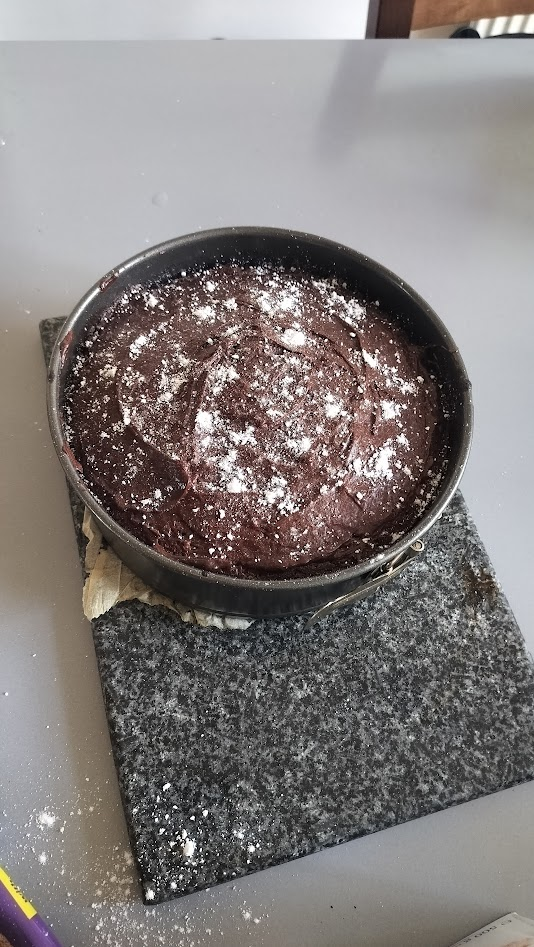
\includegraphics[width=\paperwidth,height=\paperheight]{banankage2.jpg} };
\end{tikzpicture}
\newpage
\newpage
\chapter{Brød}
\section{Brioche}
\begin{minipage}[t]{0.5\textwidth}
\end{minipage}
\begin{minipage}[t]{0.5\textwidth}
\end{minipage}
\section{Ciabatta}
\begin{minipage}[t]{0.5\textwidth}
\end{minipage}
\begin{minipage}[t]{0.5\textwidth}
\end{minipage}
\section{Focaccia}
\begin{minipage}[t]{0.5\textwidth}
\end{minipage}
\begin{minipage}[t]{0.5\textwidth}
\end{minipage}
\newpage \section{Naan}
\begin{minipage}[t]{0.5\textwidth}
\textbf{Ingredienser:}
\begin{itemize}
    \item 1 dl stuetempereret vand
    \item25 g gær
    \item1 dl mælk
    \item1 æg, sammenpisket
    \item1 dl græsk yoghurt 10 %
    \item3 spsk olivenolie
    \item1 tsk salt
    \item1 tsk sukker
    \item450 g hvedemel
\end{itemize}
    Pensling og smag
\begin{itemize}
    \item  50 g smør, smeltet
    \item Fiske koriander, finthakket
    \item2 fed hvidløg, pressede
    \begin{enumerate}
        \item  evt 1 spsk nigella frø. \\
        Nigella frø kan fås i inco og ligende, men tilføje ikke det i forhold til smagen
    \end{enumerate}
\end{itemize}
\end{minipage}
\begin{minipage}[t]{0.5\textwidth}
\begin{enumerate}
    \item Kom vand i en skål og rør gær ud i væsken. Tilsæt mælk, æg, yoghurt, olivenolie, sukker og salt samt halvdelen af melet. 
    \item Rør det grundigt igennem og tilsæt så lidt efter lidt mere mel.Ælt dejen godt, til den er smidig, blød og stadig klistret og kom den i en skål.
    \item Dæk dejen til og lad den hæve i en times tid til omtrent dobbelt størrelse. Del dejen i 2 dele og tryk eller rul hver del flad og i dråbeform. 
    \item Læg dem på en bageplade med bagepapir, dæk dem til og lad dem hæve i et kvarters tid.
    \item Pensl brødene med smeltet smør og drys med de ønskede krydderier.
    \item Bag brødene i en forvarmet ovn ved 175 grader varmluft i cirka 20 minutter.

\end{enumerate}
\end{minipage}
\newpage \section{Pizzadej}
\begin{minipage}[t]{0.5\textwidth}
\textbf{Ingredienser:}
\begin{itemize}
    \item 25 g gær eller 5 g gær til koldhævning
    \item 2.5 dL vand
    \item 3 spsk olivenolie
    \item 1 tsk salt
    \item 500g hvedemel
\end{itemize}
\underline{Ekstra:}
    \begin{enumerate}
        \item  1 spsk olivenolie til smøring
        \item Masser af mel til udrulning
    \end{enumerate}
\end{minipage}
\begin{minipage}[t]{0.5\textwidth}
\textbf{Fremgangsmåde:}
\begin{enumerate}
    \item Bland gæren med lunkent vand, 25 gram til ~1 times hævning og 5g til koldhævning
    \item Kom 1/3 af melen i, olivenolien og salt i og rør til ens konsistens, dernæst tilføj det sidste mel lidt efter lidt
    \item Drys mel på bordet og ælt dejen til smidig. Olier en skål og kom dejen i, tildæk med viskestykke og lad hæve i 1 time eller natten over
    \item Til sidst kan dejen med fordell deles i 2, så der kan laves med 2 forskellige slags fyld, bag i 250 C° forvarmet ovn i cirka 10 minutter 
\end{enumerate}
\end{minipage}
\chapter{Drinks}

\end{document}
